%\documentclass[landscape,a0b,final,a4resizeable]{a0poster}
% \documentclass[landscape,a0b,final]{a0poster}
\documentclass[landscape,a0b,final]{a0poster}
%\setlength{\paperwidth}{48in}
%\setlength{\paperheight}{36in}
%\setlength{\textwidth}{20in}
%\setlength{\textheight}{50in}

%\setlength{\textwidth}{15in}
%\setlength{\textheight}{20in} 
% \documentclass[portrait,a0b,final,a4resizeable]{a0poster}
% \documentclass[portrait,a0b,final]{a0poster}
%%% Option "a4resizeable" makes it possible ot resize the
% poster by the command: psresize -pa4 poster.ps poster-a4.ps
% For final printing, please remove option "a4resizeable" !!

%\usepackage{epsfig}
\usepackage{multicol}                                           %Multiple Columns
\usepackage[left=1cm,right=1cm,bottom=1cm,top=1cm]{geometry}	%Reset margins
\usepackage{times,amsmath,float,color}
\usepackage{graphicx} 
\usepackage{hhline}
\usepackage{natbib}
\usepackage[T1]{fontenc}			%Need for gtamac fonts
\usepackage{textcomp}
\usepackage{mathpazo}			%Load palatino font & pazo math
\usepackage{times}
\usepackage{wrapfig}
\bibliographystyle{/Users/hpmarshall/D_DRIVE/latex/agu} 
%\usepackage{tabular}
%\usepackage[large]{subfigure} 
%\usepackage[latin1]{inputenc}
%\usepackage[font=scriptsize,bf]{caption}
\DeclareGraphicsRule{.tif}{png}{.png}{`convert #1 `dirname #1`/`basename #1 .tif`.png}

\def\sA{{\mathcal{A}}}
\def\sB{{\mathcal{B}}}

%%%%%%%%%%%%%%%%%%%%%%%%%%%%%%%%%%%%%%%%%%% 
% Definition of some variables and colors
%%%%%%%%%%%%%%%%%%%%%%%%%%%%%%%%%%%%%%%%%%

% \renewcommand{\rho}{\varrho}
% \renewcommand{\phi}{\varphi}
\setlength{\columnsep}{3cm}                     %Set spacing between columns
\setlength{\columnseprule}{2mm}                 %lines as column separators
\setlength{\parindent}{0.0cm}

%%%Define colours and lengths
\definecolor{headingcol}{rgb}{1,0.7,0}		%Color of main title
\definecolor{fillcol}{rgb}{0.9,0.9,1}	        %Fill-color of box
\definecolor{boxcol}{rgb}{0.2,0.2,0.5}		%Edge-color of box and top banner
\fboxsep=0.5cm					%Padding between box and text
\fboxrule=1.5mm					%Width of box outline
\renewcommand{\rmdefault}{ppl}			%Reset serif to Palatino

% Figures within a column:
\makeatletter
\newenvironment{tablehere}
{\def\@captype{table}}
{}
\newenvironment{figurehere}
{\def\@captype{figure}}
{}
\makeatother

% changing the font of the caption, to make it stick out
%\usepackage[font=sf]{caption}
%\setlength{\belowcaptionskip}{15pt}

%%% Format title
\makeatletter				%Needed to include code in main file
\renewcommand\@maketitle{%
\null					%Sets position marker
{
\color{headingcol}\sffamily\veryHuge	%Set title font and color (from above)
\@title \par}%
\vskip 0.6em%
{
\color{white}\sffamily\large		%Set author font and color(white)
\lineskip .5em%
\begin{tabular}[t]{l}%
\@author
\end{tabular}\par}%
\vskip 1cm
\par
}
\makeatother

\newsavebox\envbox 			%Define name for boxes used

%%%%%%%%%%%%%%%%%%%%%%%%%%%%%%%%%%%%%%%%%%%%%%%%%%
%%% Define "Section" environment for framed boxes
%%% Usage: \begin{Section}{Name} blah blah blah \end{Section}
%%%%%%%%%%%%%%%%%%%%%%%%%%%%%%%%%%%%%%%%%%%%%%%%%

\newenvironment{sectionbox}[1]		%Environment takes one argument
%%%Opening
{
\par 
\flushleft
\colorbox{boxcol}{ 				%Draws solid color box around title
\sffamily\Large \color{white} #1                %Typesets section name
\hspace{0.5cm}}
\par\nobreak 
\nointerlineskip 				%Fits title snugly above box (no gap)
\setlength\parskip{-1pt}			%Even snugger
\begin{lrbox}\envbox				%Opens box environment
\begin{minipage}{0.9\columnwidth}		%Opens minipage environment for section contents
}
%%%Closing
{\par
\end{minipage}\end{lrbox}			%Close minipage and box
\fcolorbox{boxcol}{fillcol}{\usebox\envbox}	%Draw box with contents frame color: boxcol, fill color: fillcol
\vspace{1cm}					%Add spacing below box
} 

%%% This will just create a section title with no box but with horizontal line
\newenvironment{mysection}[1]		%Environment takes one argument
%%%Opening
{
\vspace{\fboxsep}                                    %Create space between area above
\par
\colorbox{boxcol}{ 				%Draws solid color box around title
\sffamily\Large \color{white} #1                %Typesets section name
\hspace{0.5cm}}
\par\nobreak 
\nointerlineskip 				%Fits title snugly above box (no gap)
\vspace{-\fboxsep}
{\color{boxcol}\rule{1\linewidth}{\fboxrule}}
\vspace{\fboxsep}                                 %Space below line and text
}


%%%%%%%%%%%%%%%%%%%%%%%
%%% Poster                                       %%%
%%%%%%%%%%%%%%%%%%%%%%%
% create a poster size that is just smaller than the
% text width to ensure the margins
\newenvironment{poster}{
  \begin{center}
    \begin{minipage}[c]{0.98\textwidth}
    }{
    \end{minipage} 
  \end{center}
}

%%%%%%%%%%%%%%%%%%%%%%%%%
%%% symbols for author affiliations              %%%
%%%%%%%%%%%%%%%%%%%%%%%%%     
\def\thefootnote{\fnsymbol{footnote}}

%%%%%%%%%%%%%%%%%%%%%%%%%
%%% Add authors and affiliations                %%%
%%%%%%%%%%%%%%%%%%%%%%%%%
 
\title{C35E-0919 : Avalanches in L-band InSAR imagery during the 2020-21 SnowEx Mission}
% \vspace{0.5cm}
\author{ \LARGE{Hans-Peter Marshall$^{1*}$, Zach Keskinen$^{1}$, Jeff Johnson$^{1}$, Scott Havens$^{2}$, Jack Tarricone$^3$, Eli Deeb$^4$, Jewell Lund$^5,6$, Rick Forster$^6$}\\ % \vspace{0.2cm}
\textbf{1} \textit{Cryosphere Geophysics And Remote Sensing (CryoGARS) lab and Department of Geosciences, Boise State University} \\
\textbf{2} \textit{Snowbound Solutions LLC} \\
\textbf{3} \textit{Department of Geography, University of Nevada Reno}
\textbf{4} \textit{U.S. Army Cold Regions Research and Engineering Laboratory} \\
\textbf{5} \textit{Cooperative Institute for Research in the Atmosphere, Colorado State University} \\
\textbf{6} \textit{Department of Geography, University of Utah} \\
\textbf{*} \textit{email: hpmarshall@boisestate.edu, earth.boisestate.edu/cryogars}}

%, , \\
%}}
%\vspace{0.5cm}
%\textbf{1} Center for Geophysical Investigations of the Shallow Subsurface, Boise State University, Boise, ID, USA}
%\title{{\bf C31A-0600:}Inversion of FMCW radar with a priori information from SMP measurements\vspace{0.5cm}}
%\author{\LARGE{Scott Havens\footnotemark[1], Hans-Peter Marshall\footnotemark[1], and John Bradford\footnotemark[1]}\\
%\Large{\footnotemark[1] \hspace{3mm} Center for Geophysical Investigations of the Shallow Subsurface, Boise State University, Boise, ID, USA}}


%%%%%%%%%%%%%%%%%%%%%%%%%%%%%%%%%%%%%%%%%%
%%% Begin of Document
%%%%%%%%%%%%%%%%%%%%%%%%%%%%%%%%%%%%%%%%%%

\begin{document}

\floatplacement{figure}{H} 

%\hspace{-2cm}			%Align with edge of page, not margin
\colorbox{boxcol}{		%Colored banner across top
\begin{minipage}[c]{0.8525\textwidth}	%Minipage for title contents
%\vspace{-3cm}			%Shift up over header image
\maketitle
\end{minipage}

% Right logos
\begin{minipage}[c]{0.15\textwidth}
\begin{flushright}

\includegraphics[height=5.5cm]{CRRELlogo.png} \hspace{0.2cm} % 
\includegraphics[height=5.5cm]{USFS_RMRS_logo.png} \hspace{0.2cm} \\

\includegraphics[height=5.5cm]{SnowExLogo.png} \vspace{0.2cm} \\
%
\includegraphics[height=5.5cm]{CRRELlogo.png} \hspace{0.2cm} \\ % 
\includegraphics[height=5.5cm]{USFS_RMRS_logo.png} \hspace{0.2cm} \\
%
\includegraphics[height=5.5cm]{NASA.pdf} \vspace{0.6cm} \\ % 
\includegraphics[height=5.5cm]{GSFC_logo.jpeg} \hspace{0.2cm} 
%
\includegraphics[height=5.5cm]{OSUlogo.jpeg} \\
%
\includegraphics[height=5.5cm]{BSU.png} \hspace{0.2cm} 

\includegraphics[height=6cm]{CryoGARSlogo.eps} \\

\end{flushright}
\end{minipage}

}
\vspace{1cm}

\begin{poster}
\thispagestyle{empty}
\begin{multicols}{4}		%Use 4-column layout
%\raggedcolumns			%Don't stretch contents vertically
%\raggedbottom

%%%%%%%%%%%%%%%%%%%%% 
%%% Content
%%%%%%%%%%%%%%%%%%%%% 
  
\begin{sectionbox}{Abstract}
\normalsize{We investigate the impact of avalanches on L-band InSAR and the potential for detecting avalanches.  In January 2024, NISAR will launch, providing global L-band InSAR data at 12 day intervals.  We compare the impact of avalanches on the L-band InSAR signal for both 7-day and 14-day intervals, using airborne L-band InSAR imagery from UAVSAR, collected as part of the SnowEx 2020-21 time series campaign.  To study temporal baselines shorter than one week, a car-based L-band InSAR was used.  Future work will incorporate arrays of infrasound sensors to compare InSAR signatures to avalanche detections from the infrasound arrays.  In the future, InSAR and infrasound could be combined to provide additional information about avalanche release for avalanche forecasters.}

\end{sectionbox}

\begin{figure}
\centering
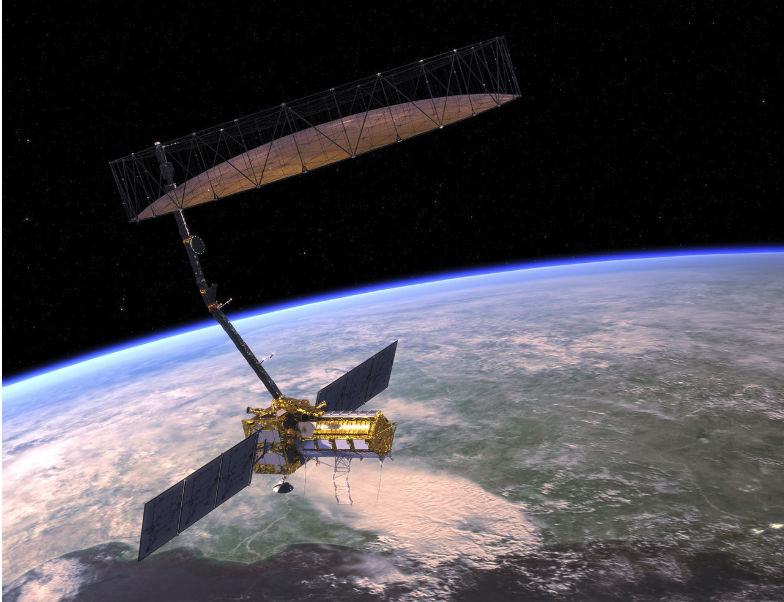
\includegraphics[width=0.8\columnwidth]{FIGURES2/NISAR.png}
\caption{NISAR launches January 2024, providing 10-50m resolution InSAR globally every 12 days.}
\label{fig:ProfileTrace} 
\end{figure}

\begin{figure}
\centering
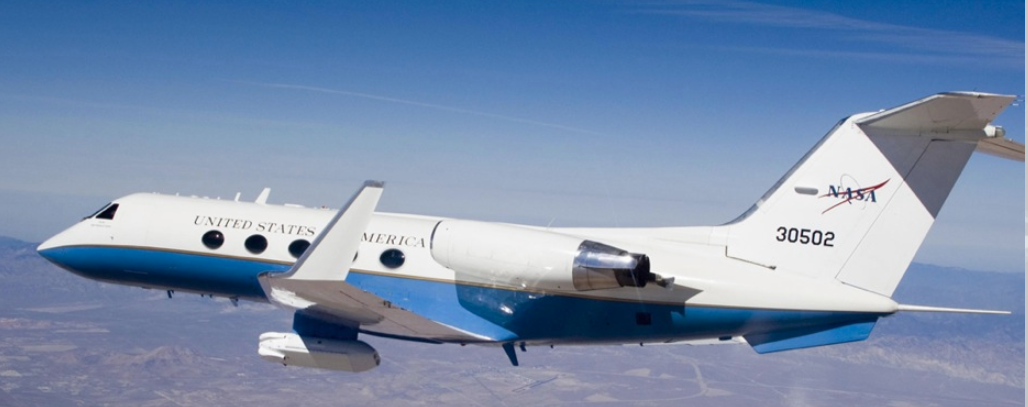
\includegraphics[width=0.8\columnwidth]{FIGURES2/UAVSAR.png}
\caption{To test the capability of NISAR for measuring snow on the ground, the 2020-21 NASA SnowEx time series was performed with UAVSAR, an airborne L-band InSAR.}
\label{fig:ProfileTrace} 
\end{figure}


\begin{mysection}{Introduction}
\vspace{-1cm}
\large{
\begin{itemize}
\item Dry snow is not expected to cause significant volume scattering at L-band frequencies ($\lambda=$24cm)       % \citep[e.g.][]{Marshall:2008}
\item If coherence is maintained, $\Delta \phi = f(H_s, SWE)$ \\ \citep{Guneriussen:2001,Deeb:2011, Marshall:2021}
\item In ideal situations avalanches can cause measurable changes in phase (Fig.~\ref{fig:InSARavy})
\end{itemize}

\begin{minipage}{1\columnwidth}
\begin{figure}
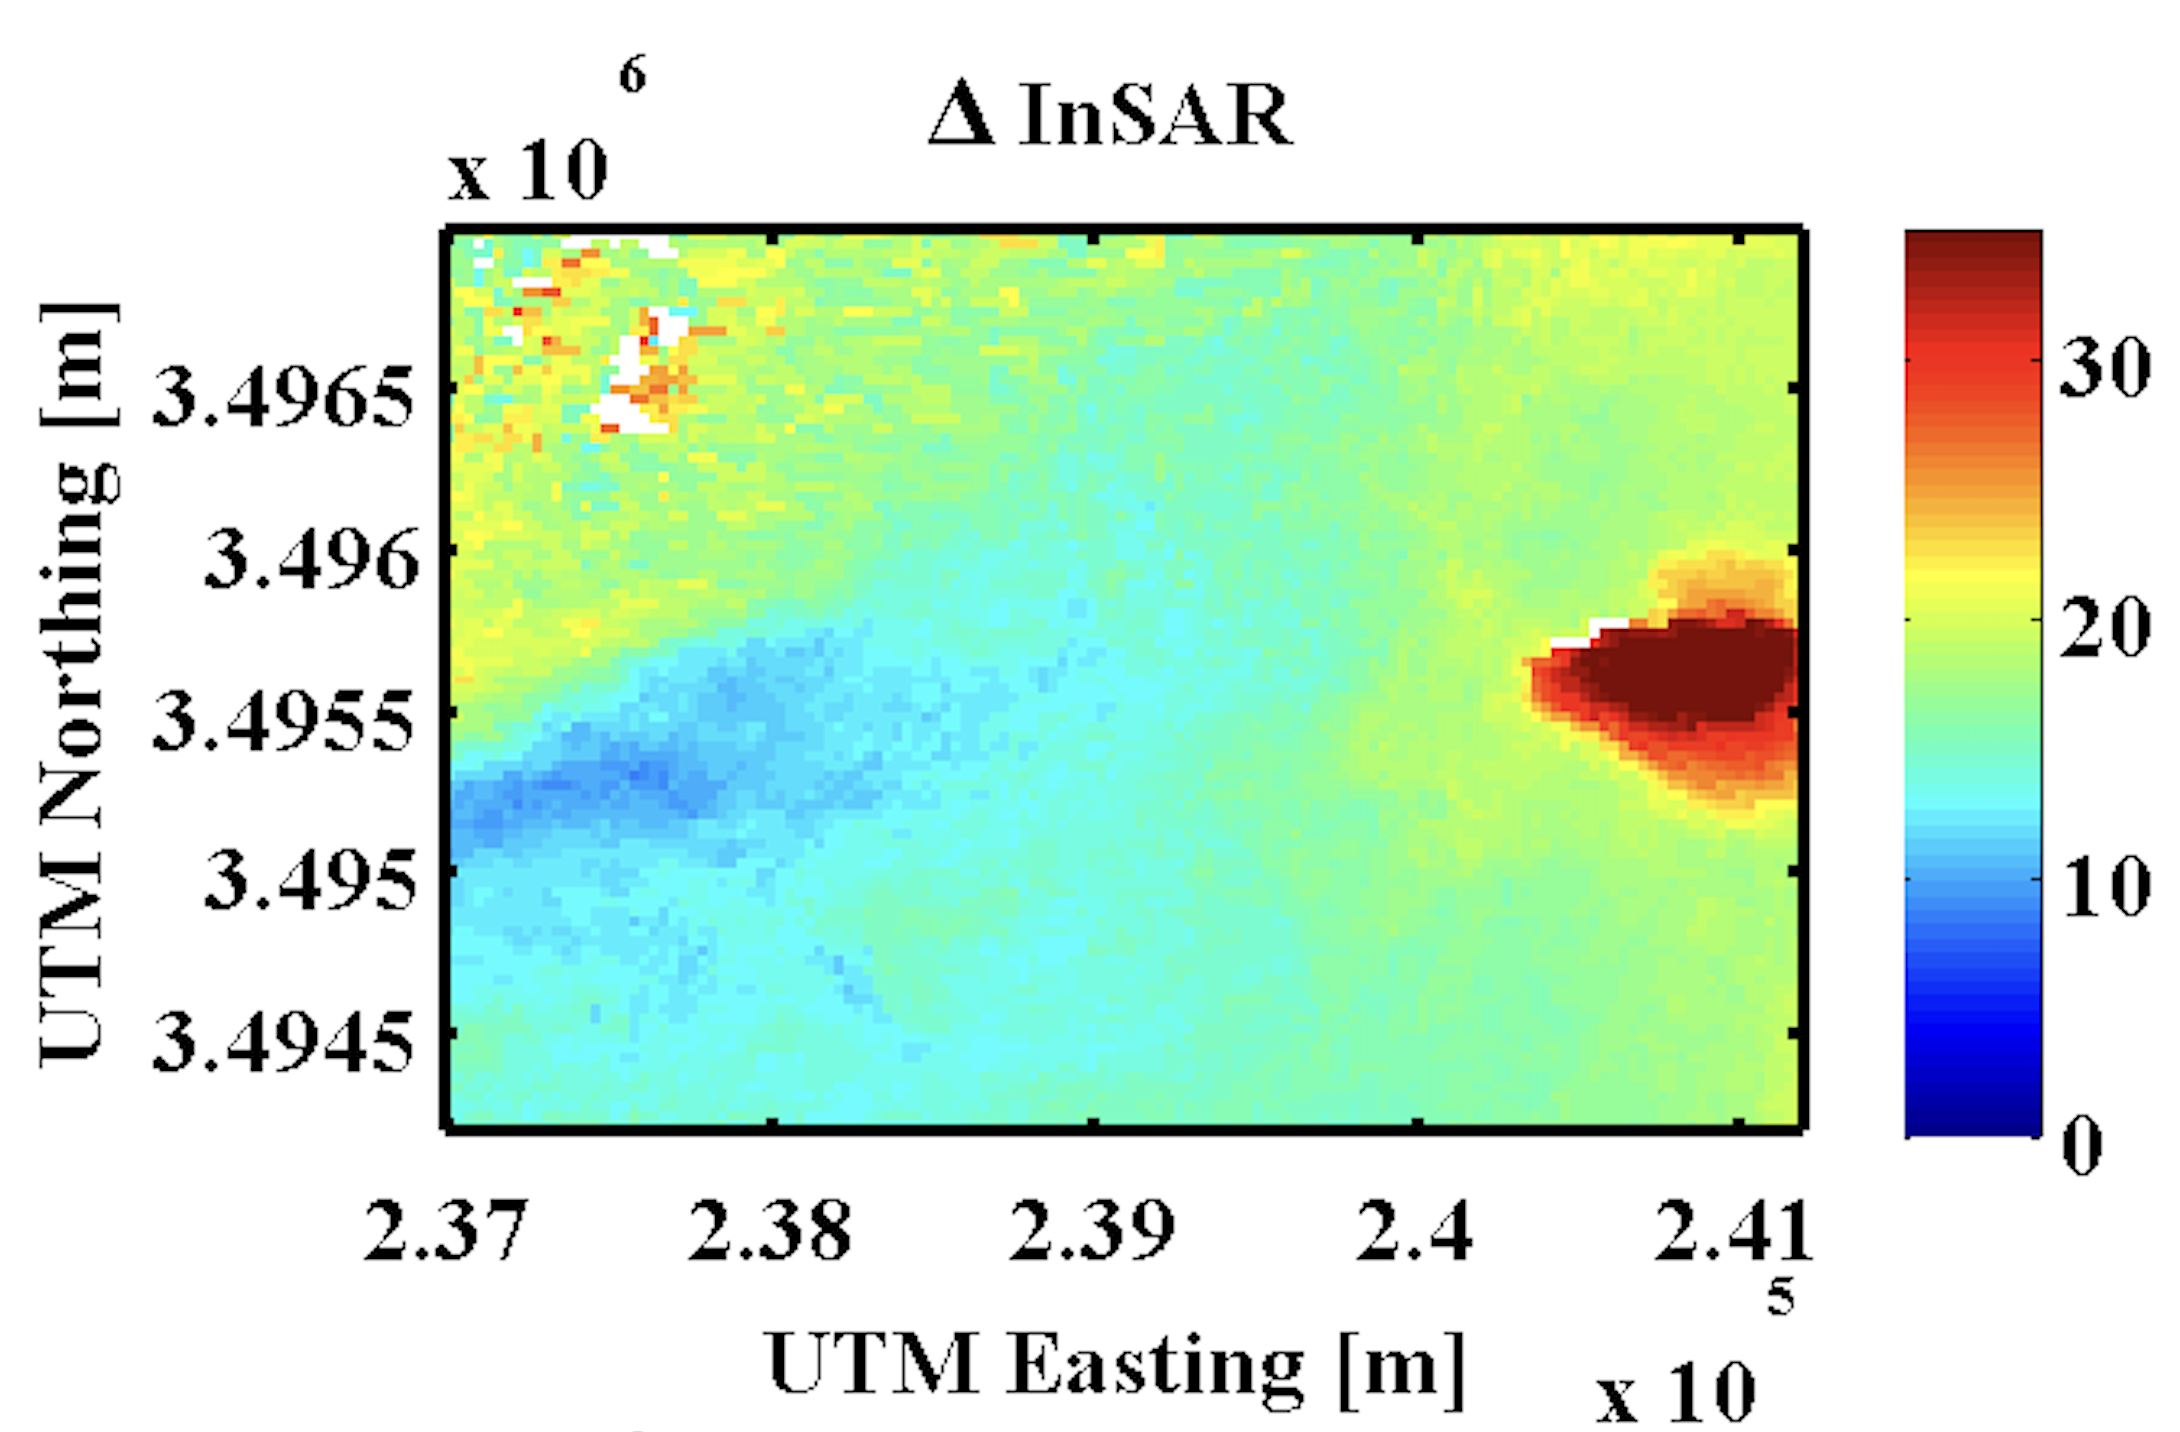
\includegraphics[width=1.05\columnwidth]{FIGURES2/InSARavy2.png}
\caption{Example of a likely avalanche in satellite L-band InSAR data (PALSAR), over High Mountain Asia.  Color shows phase change bracketing a storm, in steep mountain area with slope towards the east.}
\label{fig:InSARavy} 
\end{figure}
\end{minipage}

}
\end{mysection}

\begin{mysection}{Avalanche detection}
\large{
\begin{itemize}
\item Accurate avalanche observations are required to investigate the potential for avalanche signals in InSAR 
\item We leverage observations from avalanche forecasters, and arrays of infrasound sensors \citep{Havens:2014,Johnson:2021}
\end{itemize}


\begin{minipage}{1.05\columnwidth}
\begin{figure}
\centering
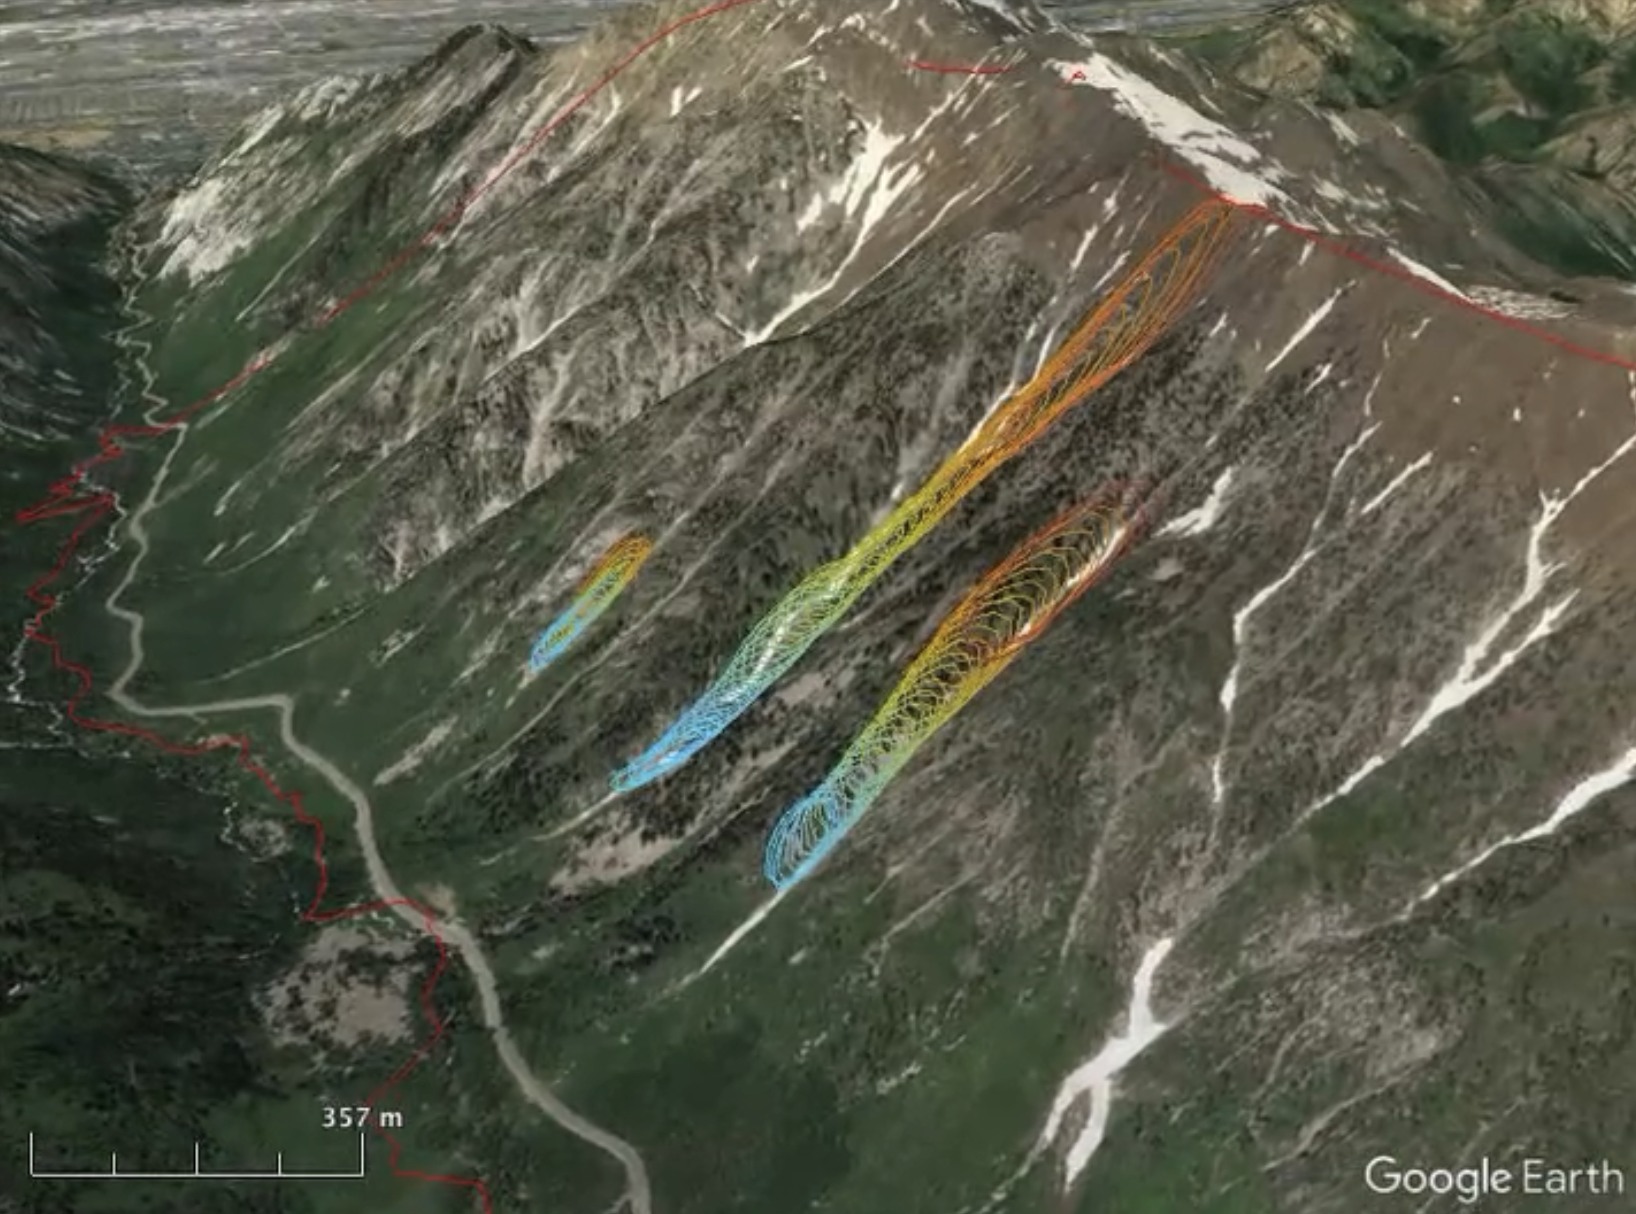
\includegraphics[width=1\columnwidth]{FIGURES2/WhitePinesAvalanches.png}
\caption{Infrasound avalanche detection, location, and tracking in LCC with multiple infrasound arrays.  Colors indicate progression of time as the avalanche
releases in the starting zone, and moves along the path \citep{Johnson:2021}}
\end{figure}
\end{minipage}
}
\end{mysection}

\begin{mysection}{Building from the ground up: CarSAR}
\vspace{-1cm}
\large{
\begin{itemize}
\item Mobile L-band InSAR allows control of temporal baseline, and enables short temporal baseline observations
\item CarSAR deployed in Little Cottonwood Canyon during SnowEx 2021, coincident w/ UAVSAR overflights
\item Changes in coherence correlated with locations where avalanche control was performed with small releases
\end{itemize}

\begin{minipage}{1\columnwidth}
\begin{figure}
\centering
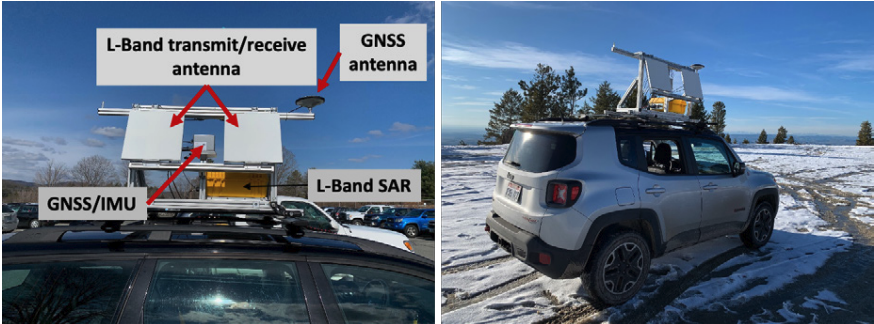
\includegraphics[width=1\columnwidth]{FIGURES2/CarSAR.png}
\caption{Mobile L-band InSAR, built by GAMMA Remote Sensing, deployed on a car.}
\end{figure}
\end{minipage}

\begin{minipage}{1\columnwidth}
\begin{figure}
\centering
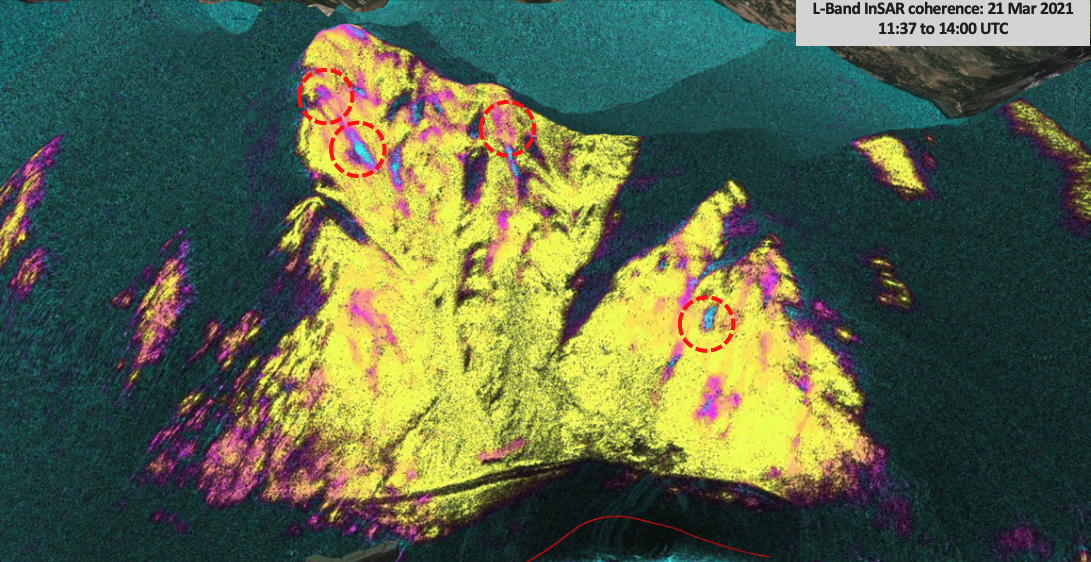
\includegraphics[width=1\columnwidth]{FIGURES2/InSARavyControl.png}
\caption{Changes in InSAR coherence indicate areas where avalanche control work was performed.}
\end{figure}
\end{minipage}

}
\end{mysection}

\begin{mysection}{Airborne L-band InSAR during SnowEx}
\vspace{-1cm}
\large{
\begin{itemize}
\item Depth change inversion from InSAR: $-\Delta H_s$ in path, $+\Delta H_s$ in debris
\item InSAR inversion shows signature of avalanches in dry snow conditions
\item Previous SAR avalanche detection has focused on changes in amplitude, and allows detection of large (>D2) slides, but small avalanches are challenging
\item InSAR phase and coherence in the right conditions may provide more sensitivity, in particular detection of smaller slides
\item Our future work will combine phase, coherence, and amplitude for detection of a wide range of avalanche sizes, using infrasound arrays to precisely determine timing and location of events
\end{itemize}

\begin{minipage}{1\columnwidth}
\begin{figure}
\centering
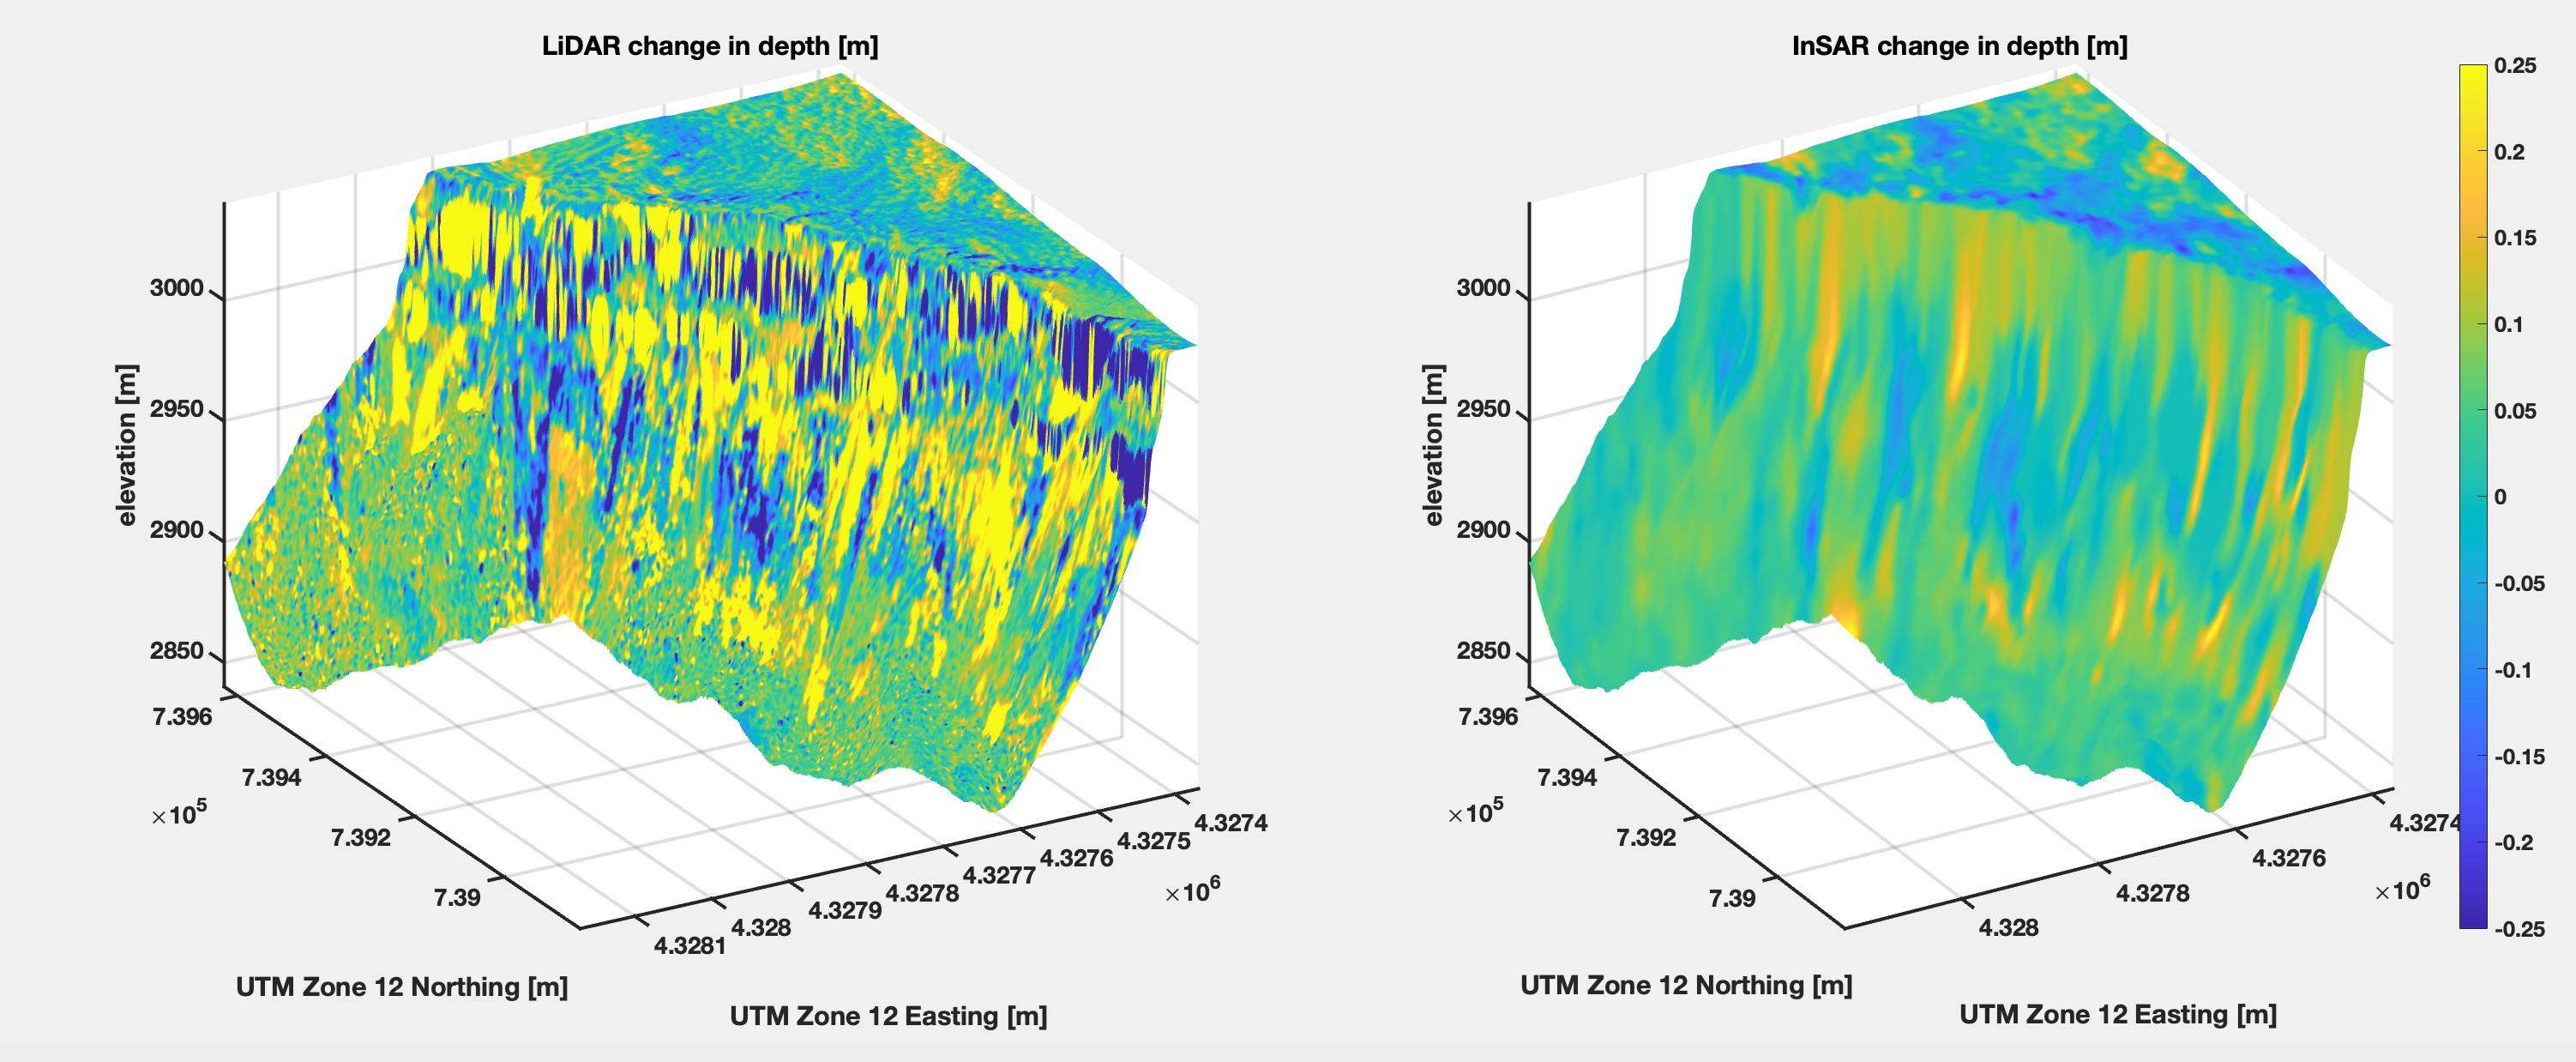
\includegraphics[width=1\columnwidth]{FIGURES2/InSAR_LiDAR_avys.png}
\caption{Dry snow avalanches on steep north-facing slopes, Grand Mesa, CO.  Depth difference during 1$^{st}$ two weeks of Feb 2020, observed by LiDAR (left) and InSAR (right) }
\end{figure}
\end{minipage}

\begin{minipage}{1\columnwidth}
\begin{figure}
\centering
\includegraphics[width=1\columnwidth]{FIGURES2/UAVSARavy.png}
\caption{UAVSAR PolSAR image over LCC (red=HH,green=HV,blue=VV) for Feb 23, 2021, after a large avalanche cycle.  Impact of avalanche debris can be seen as dark areas in runout zone.}
\end{figure}
\end{minipage}

%\begin{minipage}{0.5\columnwidth}
%\begin{figure}
%\centering
%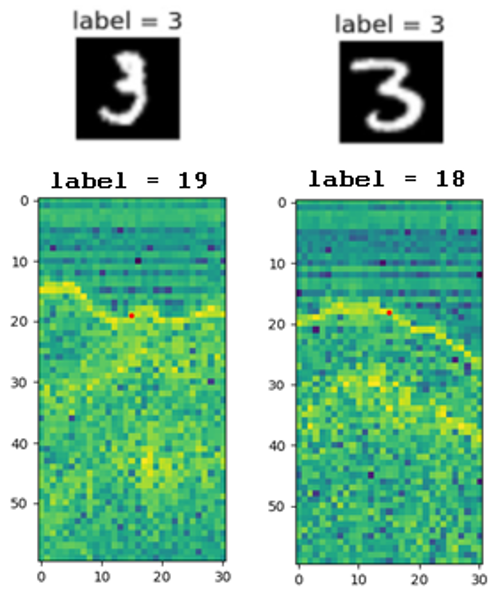
\includegraphics[width=1\columnwidth]{FIGURES/CNN.png}
%\caption{\small{}}
%\end{figure}
%\end{minipage}
%
%\begin{minipage}{1\columnwidth}
%\begin{figure}
%\centering
%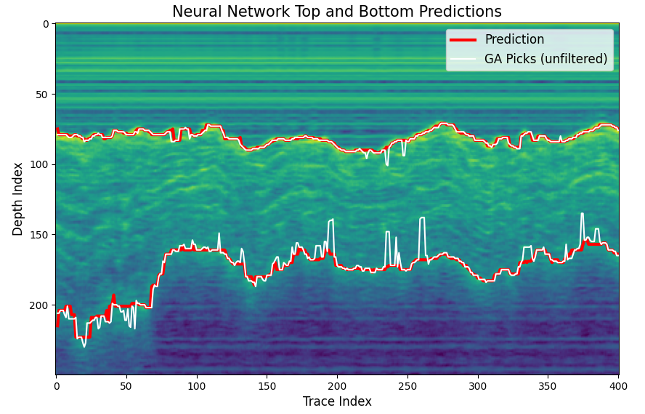
\includegraphics[width=1\columnwidth]{FIGURES/NeuralNetPicks.png}
%\caption{Genetic algorithm picks (white), used as training for neural network (picks shown in red).}
%\end{figure}
%\end{minipage}

}
\end{mysection}
%
%\begin{mysection}{Validation: Comparison to manual probe depth}
%\vspace{-1cm}
%\large{
%\begin{itemize}
%\item Comparisons made at 24 pits where radar drove same spiral coincident with manual probe measurements
%\item Similar to previous studies \citep{McGrath:2019,Webb:2020}, manual probes are deeper, likely due to over probing
%\item Comparison of mean depth across 24 pit sites, not used for training, shows good agreement (r=0.95, RMSE<5cm) with automatic picking
%\end{itemize}
%
%\begin{minipage}{1\columnwidth}
%\begin{figure}
%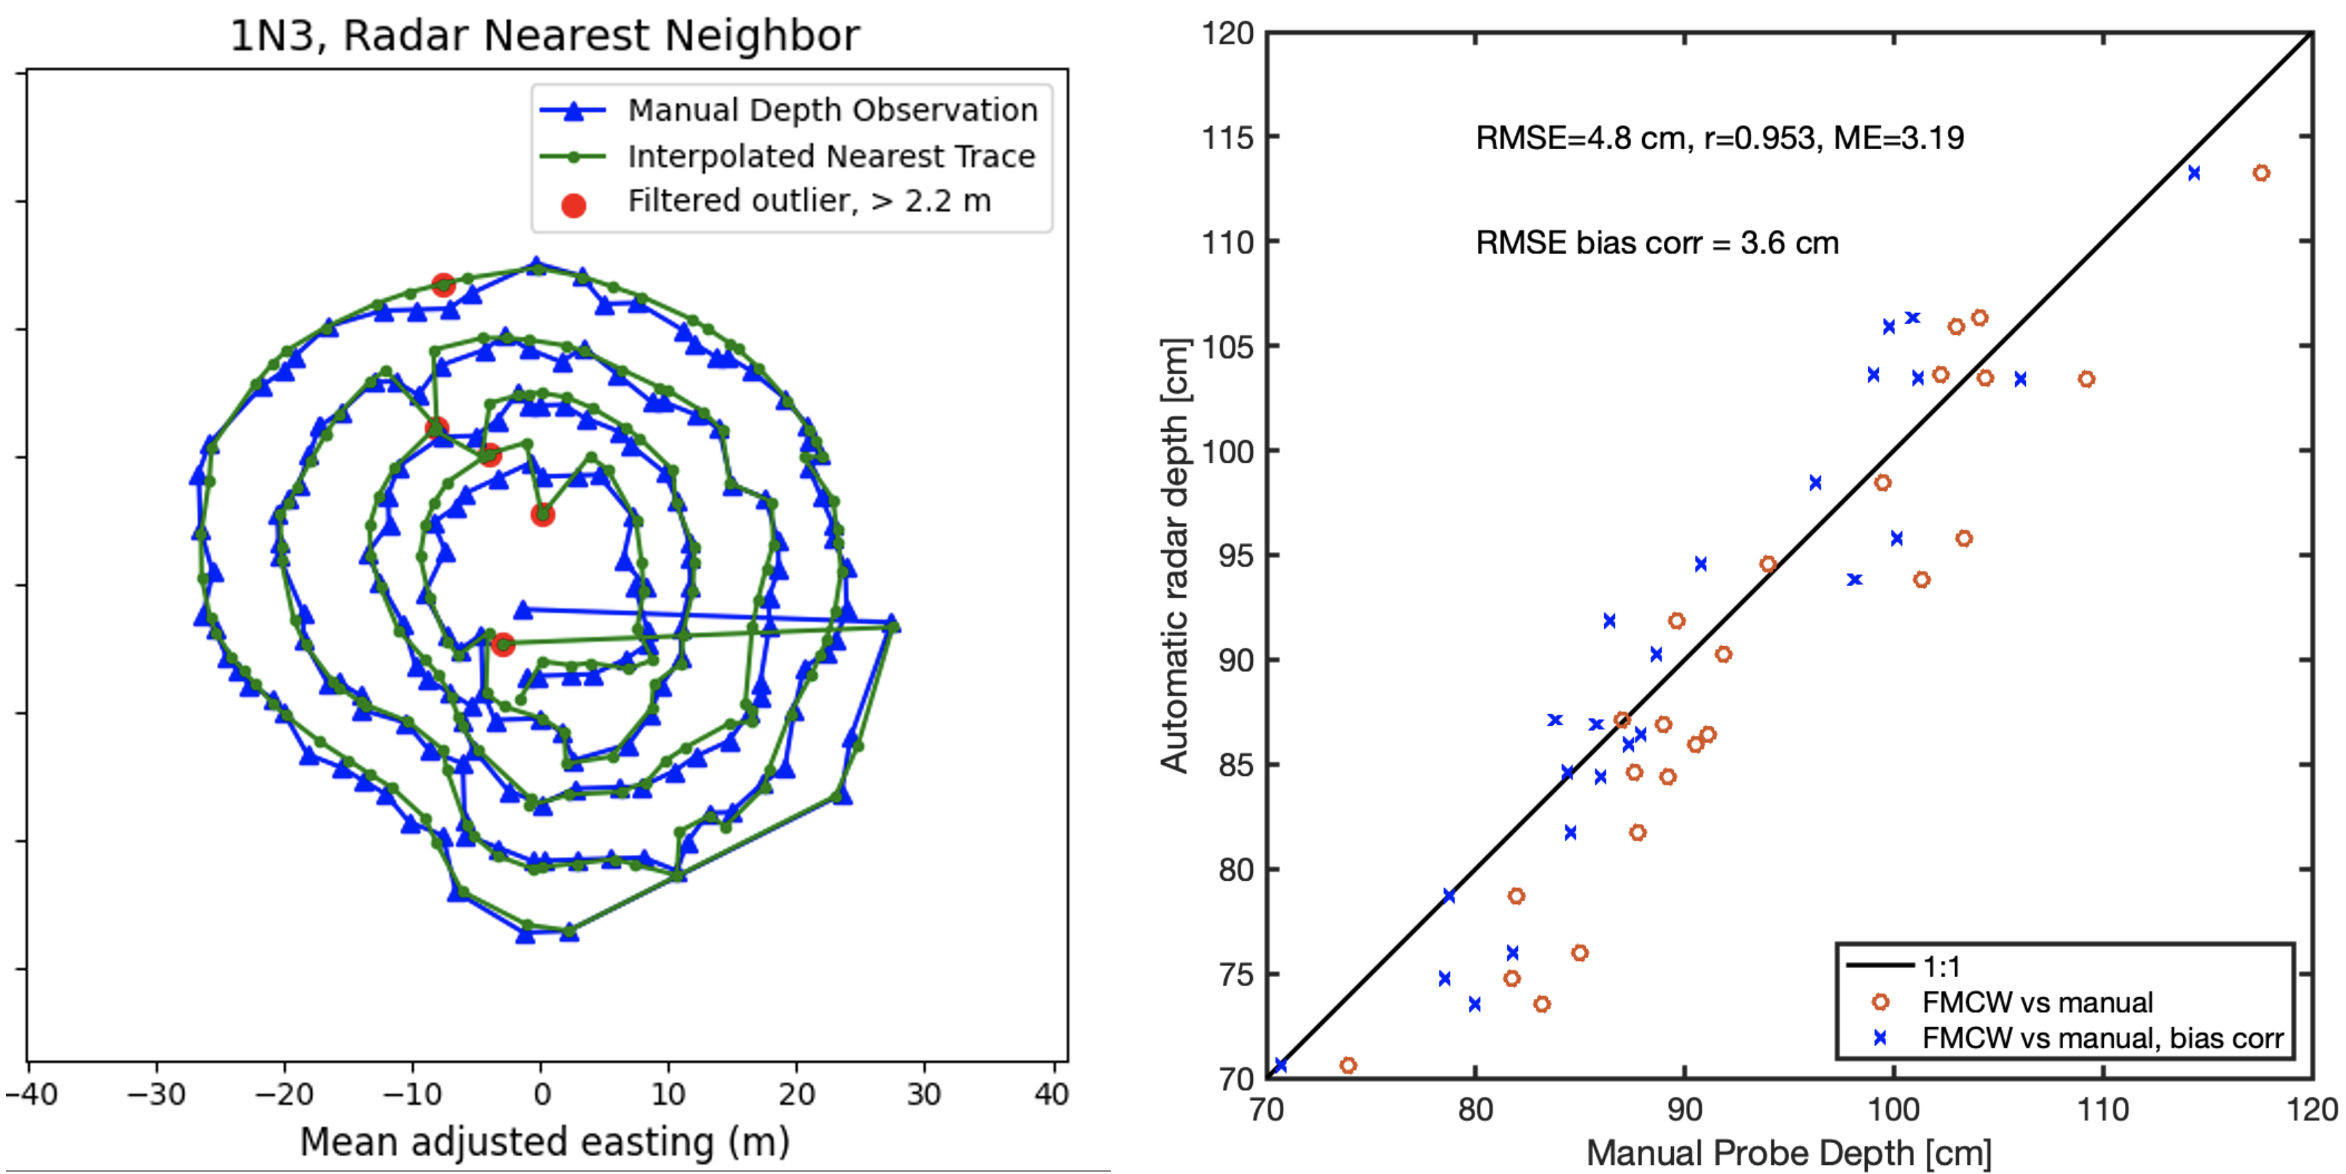
\includegraphics[width=1\columnwidth]{FIGURES/SpiralCompare.png}
%\caption{Example spiral around snowpit, showing location of manual depth observations and radar transects (left), and a comparison of mean manual depth observations and automatic radar results at 24 test pits.}
%\end{figure}
%\end{minipage}
%
%}
%\end{mysection}
%
%\begin{mysection}{Stratigraphy Information}
%\vspace{-1cm}
%\large{
%\begin{itemize}
%\item Stratigraphy can cause challenges for active and passive microwave retrievals of snow
%\item Random forest used to classify radar profiles into high stratigraphy and low stratigraphy regions
%\end{itemize}
%
%\begin{minipage}{1\columnwidth}
%\begin{figure}
%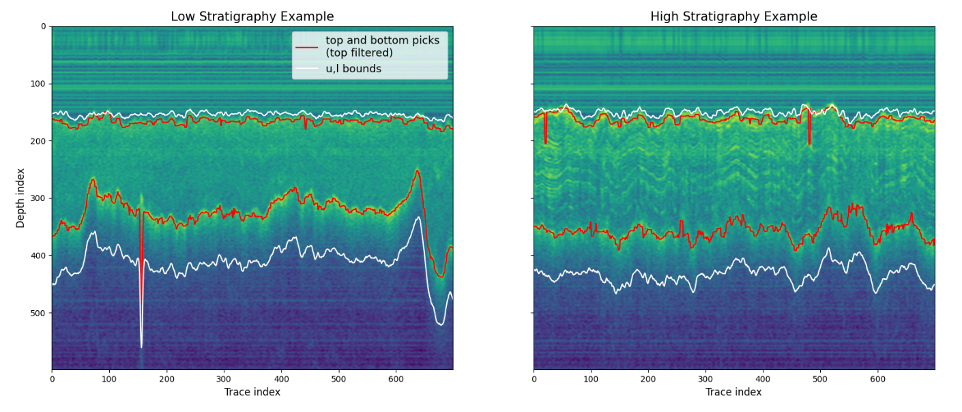
\includegraphics[width=1\columnwidth]{FIGURES/Stratigraphy.png}
%\caption{Random forest classified radar transects as either low stratigraphy (left) or high stratigraphy (right).}
%\end{figure}
%\end{minipage}
%
%}
%\end{mysection}
%

%\begin{mysection}{Depth change and total depth, compared to in-situ observations}
%\vspace{-1cm}
%\large{
%\begin{itemize}
%\item 
%\end{itemize}
%
%\begin{minipage}{1\columnwidth}
%\begin{figure}
%\centering
%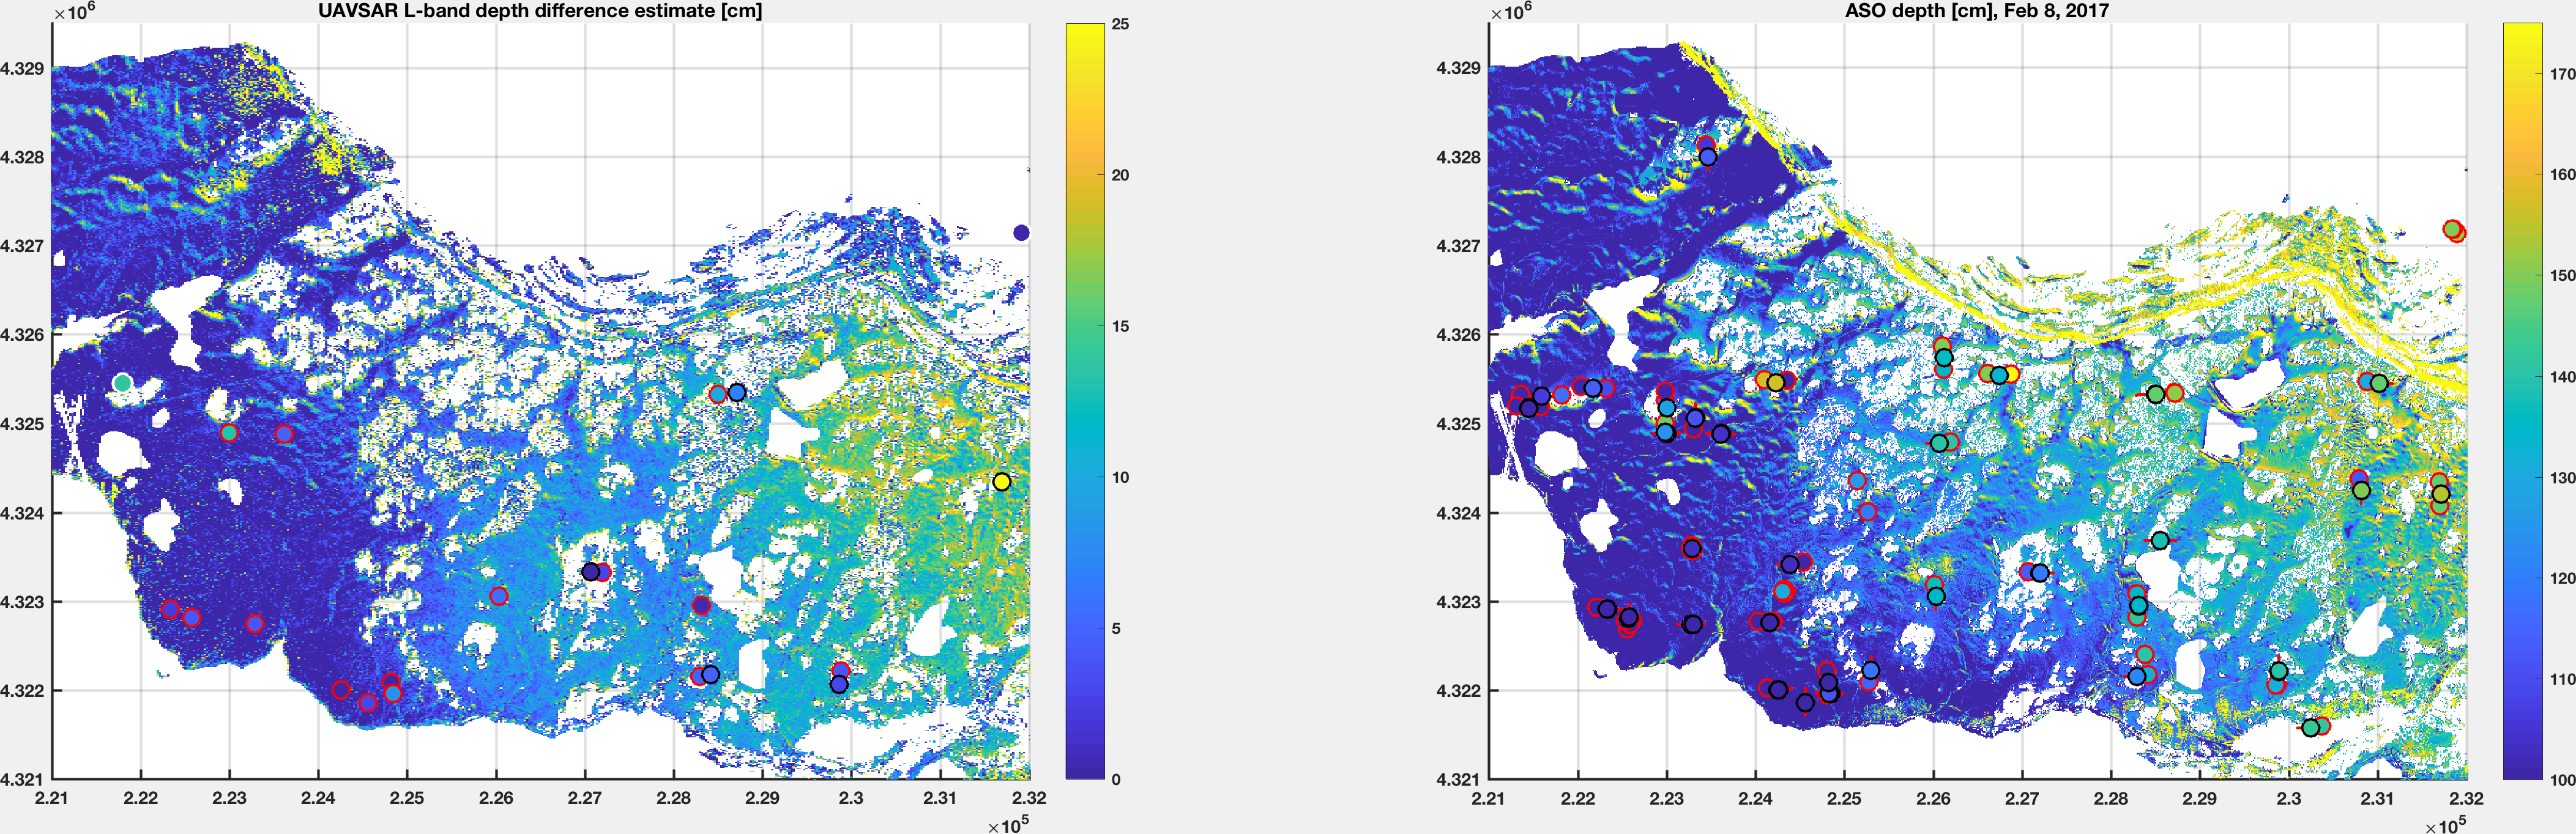
\includegraphics[width=1\columnwidth]{Fig8.png}
%\caption{\small{Left: InSAR depth estimate, with in-situ depth changes shown with filled circles.  Right: LiDAR snow depth, with in-situ depths shown with filled circles.}}
%\label{fig:InSAR_LiDAR_1km} 
%\end{figure}
%\end{minipage}
%
%}
%\end{mysection}
%\begin{mysection}{InSAR depth change at 1 km$^2$ scale}
%\vspace{-1cm}
%\large{
%\begin{itemize}
%\item 
%\end{itemize}
%
%\begin{minipage}{1\columnwidth}
%\begin{figure}
%\centering
%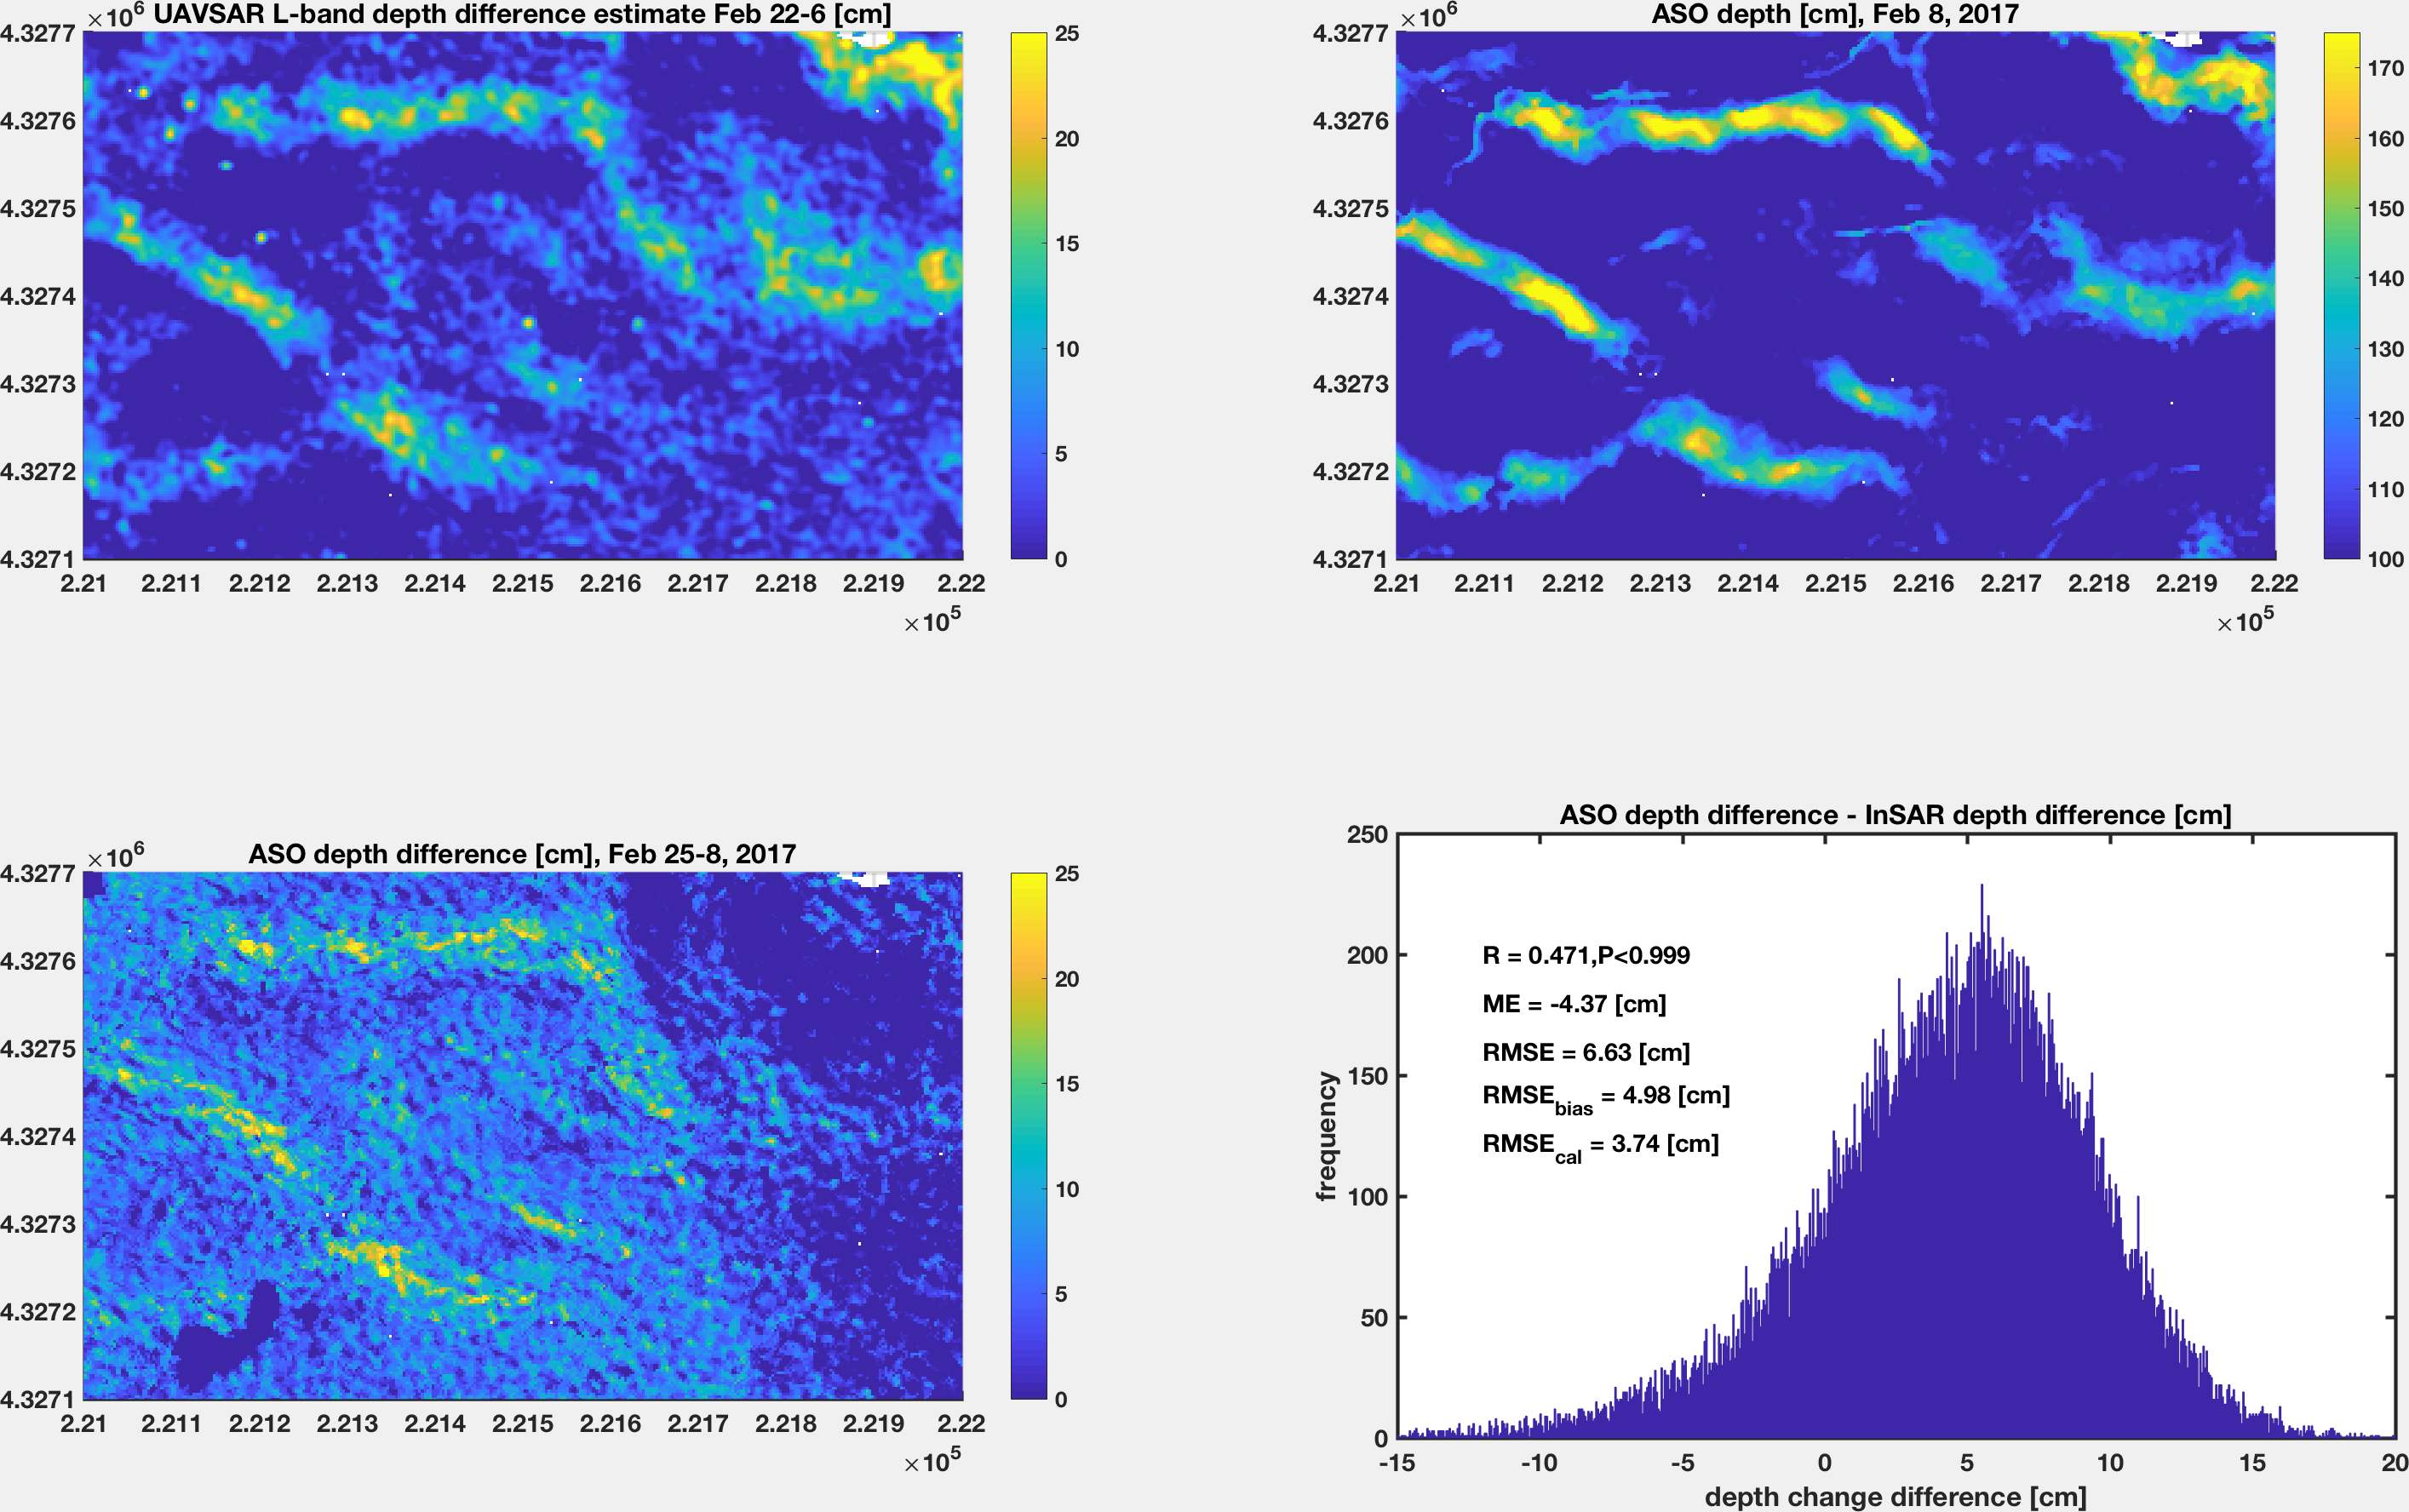
\includegraphics[width=1\columnwidth]{Fig9.png}
%\caption{\small{Top left: InSAR depth change retrieval. Top right: LiDAR snow depth.  Bottom left: LiDAR depth change.  Bottom right: histogram of LiDAR-InSAR depth change.}}
%\label{fig:InSAR_LiDAR_1km} 
%\end{figure}
%\end{minipage}

%}
%\end{mysection}


%\large{
%\begin{minipage}{0.6\columnwidth}
%\begin{figure}
%  \begin{center}
%   \includegraphics[width=1\columnwidth]{FMCWinsitu.pdf}
%   \caption{\small{Snowpit observations, In-situ reflectivity, FMCW profile, metal reflector exp}}
%   \label{fig:multiGPR} 
%  \end{center}
% \end{figure}
%\end{minipage}
%\begin{minipage}{0.35\columnwidth}
%\begin{figure}
%  \begin{center}
%   \includegraphics[width=1\columnwidth]{Reflectivity.png}
%   \caption{\small{In-situ reflectivity vs. FMCW backscatter}}
%   \label{fig:multiGPR} 
%  \end{center}
% \end{figure}
%\end{minipage}
%
%\begin{minipage}{0.4\columnwidth}
%\begin{figure}
%  \begin{center}
%   \includegraphics[width=1\columnwidth]{InSitu.png}
%   \caption{\small{In-situ dielectric constant}}
%   \label{fig:multiGPR} 
%  \end{center}
% \end{figure}
%\end{minipage}
%\begin{minipage}{0.3\columnwidth}
%\begin{figure}
%  \begin{center}
%   \includegraphics[width=1\columnwidth]{Layers.png}
%   \caption{\small{Arctic snow stratigraphy}}
%   \label{fig:multiGPR} 
%  \end{center}
% \end{figure}
%\end{minipage}
%\begin{minipage}{0.3\columnwidth}
%\begin{figure}
%  \begin{center}
%   \includegraphics[width=1\columnwidth]{LayerVar.png}
%   \caption{\small{Layer variation in three parallel trenches over 50cm}}
%   \label{fig:multiGPR} 
%  \end{center}
% \end{figure}
%\end{minipage}
%
%\begin{minipage}{0.65\columnwidth}
%\begin{itemize}
%\item Continuous reflections caused by density changes at layer boundaries
%\item Cause of reflections can be confirmed with metal reflection experiments
%\item Amplitude of reflection is a function of dielectric contrast
%\item Small scale variations in stratigraphy larger than variations in bulk properties
%\item Average reflectivity and average radar backscatter from layer boundaries highly correlated
%\end{itemize}
%\end{minipage}
%\begin{minipage}{0.3\columnwidth}
%\begin{figure}
%  \begin{center}
%   \includegraphics[width=1\columnwidth]{MuliGPR.pdf}
%   \caption{\small{Multi-channel radar for continuous density profiling}}
%   \label{fig:multiGPR} 
%  \end{center}
% \end{figure}
%\end{minipage}
%
%}
%\end{mysection}

%%% Conclusions %%%
%\begin{mysection}{Conclusions}
%\large{
%\begin{itemize}
%\item Variations below 500 m can be large, and high resolution observations at the km-scale are needed to understand and model snow distribution accurately
%\item High resolution (2cm vertical, 10cm horizontal) radar measurements produce detailed view of spatial distribution of depth, density, stratigraphy and density profiles at a resolution and scale not possible with traditional techniques.  
%\item Measurements at the km scale are quick and low cost, and bridge the gap between point observations and remote sensing and modeling pixel scales.
%\item Amplitude of reflections from layer boundaries are highly correlated with magnitude of density change, but require averaging many observations
%\item Multi-channel radar allows independent measurements of layer thickness and density
%\item Combining multi-channel radar with forward modeling = accurate profiles of density, layer boundaries, liquid water content 
%\end{itemize}
%
%\begin{minipage}{0.4\columnwidth}
%\begin{figure}
%  \begin{center}
%   \includegraphics[width=1\columnwidth]{DoubleRadar.jpg}
%   \label{fig:SMP_profile} 
%  \end{center}
% \end{figure}
%\end{minipage}
%\begin{minipage}{0.3\columnwidth}
%\begin{figure}
%  \begin{center}
%   \includegraphics[width=1\columnwidth]{HPAndyRadar.jpg}
%   \label{fig:SMP_profile} 
%  \end{center}
% \end{figure}
%\end{minipage}
%\begin{minipage}{0.3\columnwidth}
%\begin{figure}
%  \begin{center}
%   \includegraphics[width=1\columnwidth]{radar2.jpg}
%   \label{fig:SMP_profile} 
%  \end{center}
% \end{figure}
%\end{minipage}
%}
%\end{mysection}


\begin{mysection}{Acknowledgments}

\small{
This work was funded by the NASA Terrestrial Hydrology Program, grant \#NNX17AL61G and U.S. Army CRREL, "Advancement of snow monitoring for water resources, vehicle mobility, and hazard mitigation:
using optical, microwave, acoustic, and seismic techniques", \# W913E520C0017, and by NASA Terrestrial Hydrology Program, "Spatiotemporal Patterns in Snow Remote Sensing", \#NNX17AL61G.  The authors thank the UDOT avalanche forecasters in Little Cottonwood Canyon.

%\nocite{Deeb:2011,Engen:2004,Li:2017}

%\vspace{-2cm}
\small{
\bibliography{mypubs2,snow12}
}
}
\end{mysection}



\end{multicols}
  
%\begin{multicols}{2}
%\begin{mysection}{Km-scale profiles}
%\large{
%\begin{minipage}{0.6\columnwidth}
%\begin{figure}
%  \begin{center}
%\includegraphics[width=1\columnwidth]{SBB.png}
%\caption{\small{2-10 GHz FMCW radar measurements in the high alpine, Senator Beck Basin, CO.}}
%\label{SBB} 
%\end{center}
%\end{figure}
%\end{minipage}
%\begin{minipage}{0.3\columnwidth}
%\begin{figure}
%\begin{center}
%\includegraphics[width=1\columnwidth]{SBB2.pdf}
%\caption{\small{Map of radar profiles in Senator Beck Basin.}}
%\label{SBTOP} 
%\end{center}
%\end{figure}
%\end{minipage}
%
%\begin{figure}
%\includegraphics[width=0.95\columnwidth]{LiDAR-Scale-Resolution5.pdf}
%\caption{\small{Why high resolution matters: details at scales less than 500m are often complex, complicating ground-truth of remote sensing footprints at this scale.}}
%\label{fig:LiDARres} 
%\end{figure}
%}
%\end{mysection}
%\end{multicols}
\end{poster}

\end{document}

